\documentclass[11pt]{article}

\usepackage{sectsty}
\usepackage{graphicx}
\usepackage[T1]{fontenc}
\usepackage[french]{babel}
\usepackage{hyperref}
\usepackage{listings}
\lstset{
basicstyle=\small\ttfamily,
columns=flexible,
breaklines=true,
extendedchars=true,
literate={à}{{\`a}}1 {è}{{\`e}}1 {é}{{\'e}}1 {â}{{\^a}}1,
}
\renewcommand{\baselinestretch}{1.5} 
\usepackage[skip=10pt plus1pt, indent=0pt]{parskip}
\usepackage{multicol}
\usepackage{subcaption}

% Margins
\topmargin=-0.45in
\evensidemargin=0in
\oddsidemargin=0in
\textwidth=6.5in
\textheight=9.0in
\headsep=0.25in

\title{Outil de génération de graphiques de l'IET -- Documentation}
\author{ Dominic Rivest }
\date{\today}

\begin{document}
\maketitle	
%\pagebreak

% Optional TOC
\tableofcontents
\pagebreak

%--Paper--

\section{Fonctionnement général}

L'outil de génération de graphiques de l'IET fonctionne sur un serveur hébergé par render.com. L'outil est codé dans le langage python principalement à l'aide des librairies montréalaises Dash et Plotly. Il est hébergé à l'adresse \href{https://generateur-de-graphiques-iet.onrender.com/}{https://generateur-de-graphiques-iet.onrender.com/}.

Le code est hébergé sur GitHub à l'addresse \href{https://github.com/domrivest/genGraphIET}{https://github.com/domrivest/genGraphIET}.

\subsection{Fichiers d'entrée}
L'outil prend en entrée des fichiers texte séparés en deux portions : les métadonnées et les données. Les métadonnées définissent le titre, le type, les axes, les titres d'axe, la source et certaines options d'affichage des figures. Voici un exemple de fichier de définition d'un graphique à bandes horizontal : 

\begin{lstlisting}
    metadata;chart.title;Industrial energy use by industry (2000, 2010 and 2020)
    metadata;chart.subtitle
    metadata;chart.xLabel;PJ
    metadata;chart.yLabel
    metadata;chart.source;OEE 2023
    metadata;chart.section
    metadata;chart.type;bar.grouped.horizontal
    metadata;chart.level_1;year
    metadata;chart.level_2;sector
    metadata;chart.note;Percentages shown in the vertical axis represent the share of total energy use in the sector (total is not 100% due to rounding)
    metadata;data.source
    metadata;data.file
    data;sector;year;value
    data;Mines, carrières, extraction pétrole et gaz (40.9%);2000;505.790011
    data;Mines, carrières, extraction pétrole et gaz (40.9%);2010;974.032479
    data;Mines, carrières, extraction pétrole et gaz (40.9%);2020;1439.04142
    data;Pâtes et papiers (14.1%);2000;867.656198
    data;Pâtes et papiers (14.1%);2010;552.674536
    data;Pâtes et papiers (14.1%);2020;511.646516
    data;Autres manufacturiers (12.1%);2000;563.601817
    data;Autres manufacturiers (12.1%);2010;472.032845
    data;Autres manufacturiers (12.1%);2020;427.320113
    data;Raffinage du pétrole (7.7%);2000;342.61854
    data;Raffinage du pétrole (7.7%);2010;350.948124
    data;Raffinage du pétrole (7.7%);2020;272.4289
    data;Fonte et affinage (7.6%);2000;231.263348
    data;Fonte et affinage (7.6%);2010;238.389441
    data;Fonte et affinage (7.6%);2020;268.126911
    data;Produits chimiques (7.0%);2000;260.302
    data;Produits chimiques (7.0%);2010;248.356303
    data;Produits chimiques (7.0%);2020;245.977563
    data;Fer et acier (15.1%);2000;260.134
    data;Fer et acier (15.1%);2010;213.113026
    data;Fer et acier (15.1%);2020;179.423453
    data;Construction (2.9%);2000;51.320932
    data;Construction (2.9%);2010;73.443483
    data;Construction (2.9%);2020;102.305474
    data;Ciment (1.4%);2000;67.066
    data;Ciment (1.4%);2010;57.34161
    data;Ciment (1.4%);2020;50.731356
    data;Foresterie (0.6%);2000;17.170664
    data;Foresterie (0.6%);2010;22.318411
    data;Foresterie (0.6%);2020;21.228021
\end{lstlisting}


\subsection{Modification des paramètres généraux}
\label{subsec:modifParamGlobaux}

La définition des variables et de leurs étiquettes anglaises et françaises se fait dans le fichier \textit{colors.csv}. Il est situé dans le dossier \textit{assets} du répertoire GitHub.
Outre cela, il existe deux types de paramètres modifiables par l'utilisateur du générateur de graphiques : les paramètres modifiés dans l'application et les paramètres modifiés dans les fichiers texte directement.

Le premier type inclut les paramètres suivants :
\begin{itemize}
    \item Produire les figures en français (Booléen) : Utilise la colonne \textit{label\_fr} du fichier \textit{colors.csv} si vrai.
    \item Afficher la source lorsqu'elle est renseignée dans le fichier (Booléen) : Affiche en bas de la figure la source en taille 10 si \textit{metadata;data.source} est renseigné.
    \item Afficher le titre lorsqu'il est renseigné dans le fichier (Booléen) : Affiche au-dessus de la figure le titre si \textit{metadata;chart.title} est renseigné.
    \item Taille de police (Choix d'un entier) : Contrôle la taille des éléments texte de manière relative (ex : le titre sera toujours plus gros que les titres d'axe).
    \item Spécifier la hauteur, la largeur et la résolution des figures produites (entrées d'entiers positifs). La résolution s'applique lors du téléchargement en PNG et est un simple multiplicateur des dimensions de la figure qui ne modifie pas l'échelle des éléments. Ainsi une figure de 1000x400 pixels avec une résolution de 10 deviendra une image de 10000x4000 pixels avec la même apparence.
\end{itemize}
\vspace{0.2cm}
Bien que les paramètres par défaut font bien le travail en général, certains paramètres peuvent être modifiés en spécifiant des valeurs dans les fichiers textes propres aux figures. Il s'agit d'ajouter une ligne contenant le paramètre à modifier avec la bonne syntaxe. Des exemples sont donnés ci-dessous.

\textbf{Modifications des axes :}
\begin{itemize}
    \item Type d'axe (\textit{metadata;xaxes.type} et \textit{metadata;yaxes.type}); Valeurs possibles : ( "-" | "linear" | "log" | "date" | "category" | "multicategory" ); Défaut : "-" (S'ajuste automatiquement); Documentation : \href{https://plotly.com/python/reference/layout/xaxis/#layout-xaxis-type}{Documentation Plotly}; Exemple: \textit{metadata;xaxes.type;category}
    \item Mode de graduation (\textit{metadata;xaxes.tickmode} et \textit{metadata;yaxes.tickmode}); Valeurs possibles : ( "auto" | "linear" | "array" ); Défaut : "auto"; Documentation : \href{https://plotly.com/python/reference/layout/xaxis/#layout-xaxis-minor-tickmode}{Documentation Plotly}; Exemple: \textit{metadata;xaxes.tickmode;linear}
    \item Valeur initiale de graduation (\textit{metadata;xaxes.tick0} et \textit{metadata;yaxes.tick0}); Valeurs possibles : Nombre ou catégorie; À utiliser avec \textit{dtick}. À noter que Plotly ne laissera pas de trou dans l'axe, ainsi, si la valeur initiale commence après la donnée initiale et que l'invervalle entre les graduations est trop petit, il y aura tout de même des graduations en-deça de la valeur initiale.; Documentation : \href{https://plotly.com/python/reference/layout/xaxis/#layout-xaxis-tick0}{Documentation Plotly}; Un exemple est montré ci-bas.
    \item Delta entre les graduations (\textit{metadata;xaxes.dtick} et \textit{metadata;yaxes.dtick}); Valeurs possibles : Nombre positif; À utiliser avec \textit{tick0}; Voir la documentation pour les axes de type "log" : \href{https://plotly.com/python/reference/layout/xaxis/#layout-xaxis-dtick}{Documentation Plotly}; Un exemple est montré ci-bas.
    \item Nombre maximal de graduations sur l'axe (peut être inférieur au nombre spécifié) (\textit{metadata;xaxes.nticks} et \textit{metadata;yaxes.nticks}); Valeurs possibles : Entiers positifs; Documentation : \href{https://plotly.com/python/reference/layout/xaxis/#layout-xaxis-minor-nticks}{Documentation Plotly}; Un exemple est montré ci-bas.
    \item Valeurs de graduation spécifiques (\textit{metadata;xaxes.tickvals} et \textit{metadata;yaxes.tickvals}); Valeurs possibles : Liste de nombres ou éléments de texte séparés par une virgule; Documentation : \href{https://plotly.com/python/reference/layout/xaxis/#layout-xaxis-minor-tickvals}{Documentation Plotly}; Un exemple est montré ci-bas.
    \item Rotation des étiquettes d'axe (\textit{xaxes.tickangle} et \textit{yaxes.tickangle}); Valeurs possibles : Nombre; Change l'angle des étiquettes par rapport à l'horizontal; Documentation : \href{https://plotly.com/python/reference/layout/xaxis/#layout-xaxis-tickangle}{Documentation Plotly}; Exemple: \textit{metadata;xaxes.tickangle;90}
    \item Mode d'ajustement initial de l'amplitude des axes (\textit{xaxes.rangemode} et \textit{yaxes.rangemode}); Valeurs possibles : ( "normal" | "tozero" | "nonnegative" ); Si "normal", l'échelle est affichée en fonction des données du graphique. Si "tozero", l'échelle débute à 0. Si non négatif, l'axe affichera uniquement des valeurs positives.; Documentation : \href{https://plotly.com/python/reference/layout/yaxis/#layout-yaxis-rangemode}{Documentation Plotly}; Exemple: \textit{metadata;xaxes.rangemode;tozero}
    \item Valeurs limites des axes (\textit{xaxes.range} et \textit{yaxes.range}); Valeurs possibles : Nombre, Nombre; Fixe les valeurs minimales et maximales de l'axe.; Documentation : \href{https://plotly.com/python/reference/layout/yaxis/#layout-yaxis-range}{Documentation Plotly}; Exemple: \textit{metadata;xaxes.range;0,0.85}
\end{itemize}

\vspace{0.2cm}
\textbf{Exemple d'ajustement de la graduation d'un axe des y}

Voici le code ajouté au fichier texte du graphique pour spécifier la graduation par valeur initiale et par delta:

\begin{lstlisting}
    metadata;yaxes.tickmode;linear
    metadata;yaxes.tick0;500
    metadata;yaxes.dtick;2500
\end{lstlisting}

Voici le code ajouté au fichier texte du graphique pour spécifier la graduation pour des valeurs spécifiques :

\begin{lstlisting}
    metadata;yaxes.type;linear
    metadata;yaxes.tickvals;0,2500,7500,10000
\end{lstlisting}

La figure \ref{fig:exempleGraduation} montre la différence entre les deux méthodes.

\begin{figure}[h]
    \centering
    \begin{subfigure}{\textwidth}
      \centering
      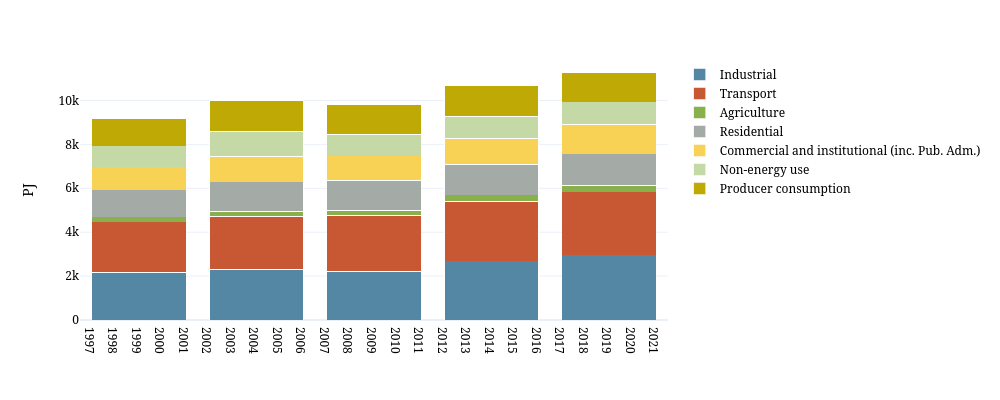
\includegraphics[width=\linewidth]{assets/fig3.2_linear_tickmode.png}
      \caption{Valeurs de graduation spécifiées par valeur initiale et par delta}
      \label{fig:grad1}
    \end{subfigure}%
    
    \begin{subfigure}{\textwidth}
      \centering
      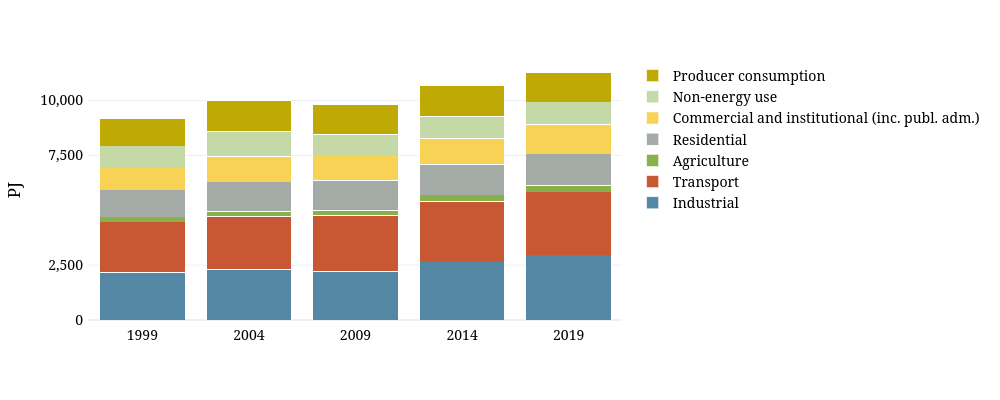
\includegraphics[width=\linewidth]{assets/fig3.2_linear_tickvals.png}
      \caption{Valeurs de graduation spécifiques}
      \label{fig:grad2}
    \end{subfigure}
    \caption{Exemple d'application des paramètres d'axe sur l'axe des y}
    \label{fig:exempleGraduation}
    \end{figure}


\pagebreak
\section{Particularité des types de graphique}

Les classes de graphique (\textit{metadata;chart.type}) présentement supportées sont les suivantes :
\begin{itemize}
    \item Graphique en aires -- \textit{area}
    \item Graphique à bandes groupées horizontal -- \textit{bar.grouped.horizontal}
    \item Graphique à bandes superposées horizontal -- \textit{bar.stacked.horizontal}
    \item Graphique à bandes superposées -- \textit{bar.stacked}
    \item Graphique à bandes groupées -- \textit{bar.grouped}
    \item Graphique à bandes superposées et groupées -- \textit{bar.grouped.stacked}
    \item Graphique à lignes -- \textit{line}
    \item Nuage de points -- \textit{scatter}
    \item Graphique en pointe de tarte -- \textit{pie}
\end{itemize}

Spécifications par type de graphique :

\textbf{Graphique en aires :}

Voici un exemple des deux premières lignes de données :
\begin{lstlisting}
    data;year;Natural gas;Crude oil;Primary electricity;Coal;Gas plant natural gas liquids (NGL's)
    data;2001;3381.3;4170.052;1364.567;1314.497;491.213
\end{lstlisting}

\textbf{Graphique à bandes groupées horizontal et graphique à bandes superposées horizontal}

Ici, la langue des variables doit être différenciée dans les fichiers texte. Voici un exemple des sept premières lignes de données :
\begin{lstlisting}
    data;usage;year;value
    data;Chauffage (56.6%);2000;603.1
    data;Chauffage (56.6%);2010;528.9
    data;Chauffage (56.6%);2020;687.8
    data;Matériel auxiliaire (15.1%);2000;87.3
    data;Matériel auxiliaire (15.1%);2010;138.1
    data;Matériel auxiliaire (15.1%);2020;183.8
\end{lstlisting}

\textbf{Graphique à bandes superposées}

Voici un exemple des trois premières lignes de données :
\begin{lstlisting}
    data;service;Electricity;Natural gas;Heating Oil;Wood;Other (including coal and propane)
    data;Space heating;260;544;52;165;14
    data;Water heating;71;197;7;5;1
\end{lstlisting}

\textbf{Graphique à bandes groupées}

Voici un exemple des trois premières lignes de données :
\begin{lstlisting}
    data;province;year;value
    data;BC;1990;15.73
    data;BC;2005;15.01
\end{lstlisting}

\textbf{Graphique à bandes superposées et groupées}

Voici un exemple des quatre premières lignes de données :
\begin{lstlisting}
    data;province;year;1990 (energy);1990 (non-energy);2005 (energy);2005 (non-energy);2021 (energy);2021 (non-energy)
    data;BC;1990;41654;10129;0;0;0;0
    data;BC;2005;0;0;50013;12960;0;0
    data;BC;2021;0;0;0;0;51814;7622
\end{lstlisting}

\textbf{Graphique à lignes et nuage de points}

Les deux types de figures se définissent de la même manière, mais le nuage de points n'a pas de lignes reliant les points. Voici un exemple des deux premières lignes de données :
\begin{lstlisting}
    data;reference;month;Mt
    data;Western Canadian Select (WCS);2014-01-01;65.69
\end{lstlisting}

\textbf{Graphique en pointe de tarte}

Pour les figures en pointe de tarte, le pourcentage par pointe est affiché par défaut. Il est cependant possible d'afficher les valeurs directement ou les deux simultanément. Cependant, cette dernière option prend plus de place dans la figure.

Voici les premières lignes de données pour le graphique par défaut :
\begin{lstlisting}
    data;Gaz;valeur;valeur %
    data;Gas_CO2;537174;80,1%
    data;Gas_CH4;90510;13,5%
\end{lstlisting}

Pour afficher la valeur uniquement (et le pourcentage dans le hover), on utilise :
\begin{lstlisting}
    metadata;chart.textinfo;value;
    metadata;chart.hoverinfo;label+percent+value;
    data;Gaz;valeur;valeur %
    data;Gas_CO2;537174;80,1%
\end{lstlisting}

Pour afficher la valeur et le pourcentage, on utilise :
\begin{lstlisting}
    metadata;chart.textinfo;value+percent;
    metadata;chart.hoverinfo;label+percent+value;
    data;Gaz;valeur;valeur %
    data;Gas_CO2;537174;80,1%
\end{lstlisting}

\begin{figure}[h]
    \centering
    \begin{subfigure}{0.49\textwidth}
        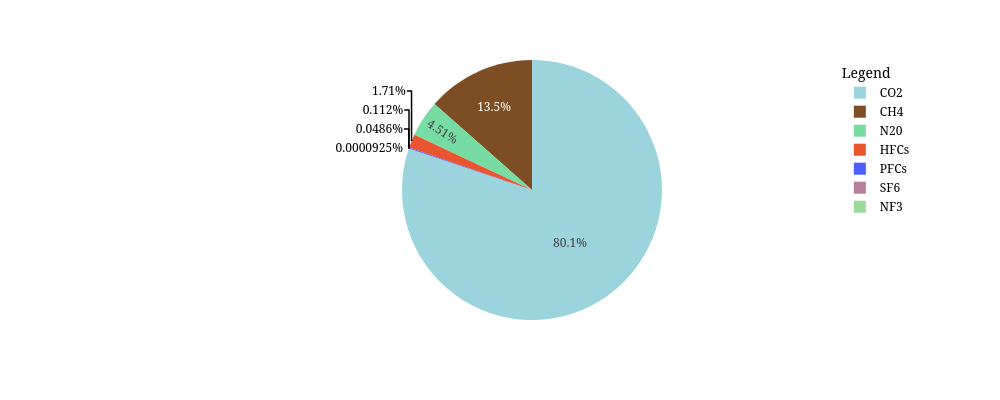
\includegraphics[width=\textwidth]{assets/fig5.2.png}
        \caption{Par défaut}
        \label{fig:firstpie}
    \end{subfigure}
    \hfill
    \begin{subfigure}{0.49\textwidth}
        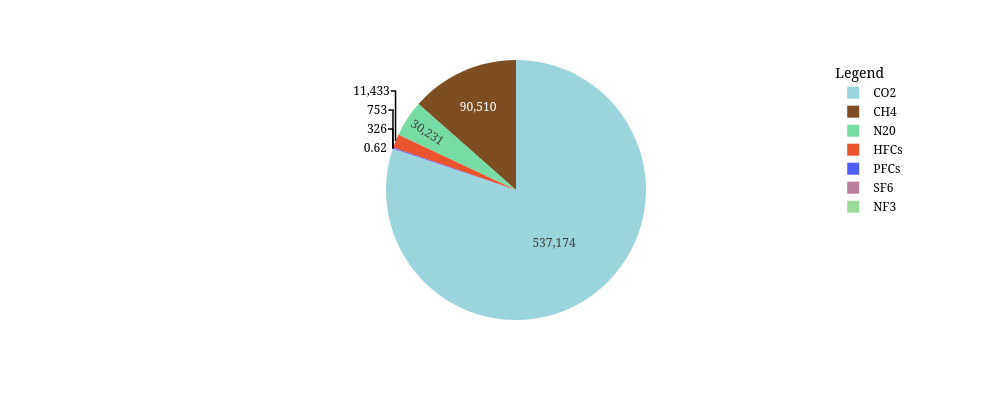
\includegraphics[width=\textwidth]{assets/fig5.2-value.png}
        \caption{Avec valeur uniquement}
        \label{fig:secondpie}
    \end{subfigure}
    \hfill
    \begin{subfigure}{0.5\textwidth}
        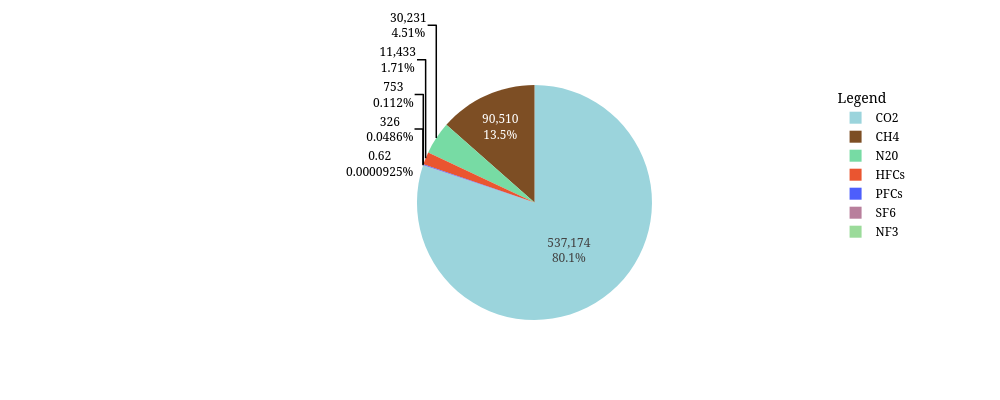
\includegraphics[width=\textwidth]{assets/fig5.2-valuePercent.png}
        \caption{Valeur et pourcentage}
        \label{fig:thirdpie}
    \end{subfigure}
            
    \caption{Configuration des figures en pointe de tarte.}
    \label{fig:piechart}
    \end{figure}

\section{Téléchargement en lot des figures affichées}

Dans l'outil de génération, le téléchargement en lot d'un maximum de 100 figures affichés est possible en format vectoriel PDF ou SVG. Dû aux limitations matérielles du serveur, à l'efficacité actuelle de la librairie d'export en PNG et à la résolution d'export souhaitée, cette option n'est pour l'instant pas disponible.

\section{Publication des figures dans \textit{Chart-Studio}}

\href{https://chart-studio.plotly.com/feed/#/}{\textit{Chart-Studio}} est une plateforme développée par \textit{Plotly} pour héberger et modifier des figures en ligne. Cette plateforme est la base de la stratégie d'intégration des figures du générateur dans Wordpress. Elle permet de conserver une copie d'un graphique sur le web et à des ressources externes comme Wordpress ou quelconque site internet d'y accéder. Le bouton d'export vers Chart-Studio envoie tous les figures affichées vers un compte Chart-Studio avec leur nom de fichier et un préfixe, si la case est remplie.

Une fois les figures exportées, on peut les retrouver sur Chart-Studio et utiliser la fonction exporter (\textit{share}) pour retrouver le code HTML ou sa version iFrame qui sera à intégrer dans la page Wordpress. Voici à quoi le code et la plateforme ressemblent lorsqu'on veut partager un graphique pour l'imbriquer :

HTML brut :
\begin{lstlisting}
    <div>
    <a href="https://plotly.com/~domrivest/186/?share_key=MPPrctkTcDTUV6joL7Ek2W" target="_blank" title="testPiefig5.2" style="display: block; text-align: center;"><img src="https://plotly.com/~domrivest/186.png?share_key=MPPrctkTcDTUV6joL7Ek2W" alt="testPiefig5.2" style="max-width: 100%;width: 1000px;"  width="1000" onerror="this.onerror=null;this.src='https://plotly.com/404.png';" /></a>
    <script data-plotly="domrivest:186" sharekey-plotly="MPPrctkTcDTUV6joL7Ek2W" src="https://plotly.com/embed.js" async></script>
</div>
\end{lstlisting}

iFrame :
\begin{lstlisting}
    <iframe width="900" height="800" frameborder="0" scrolling="no" src="//plotly.com/~domrivest/186.embed"></iframe>
\end{lstlisting}

\begin{figure}
    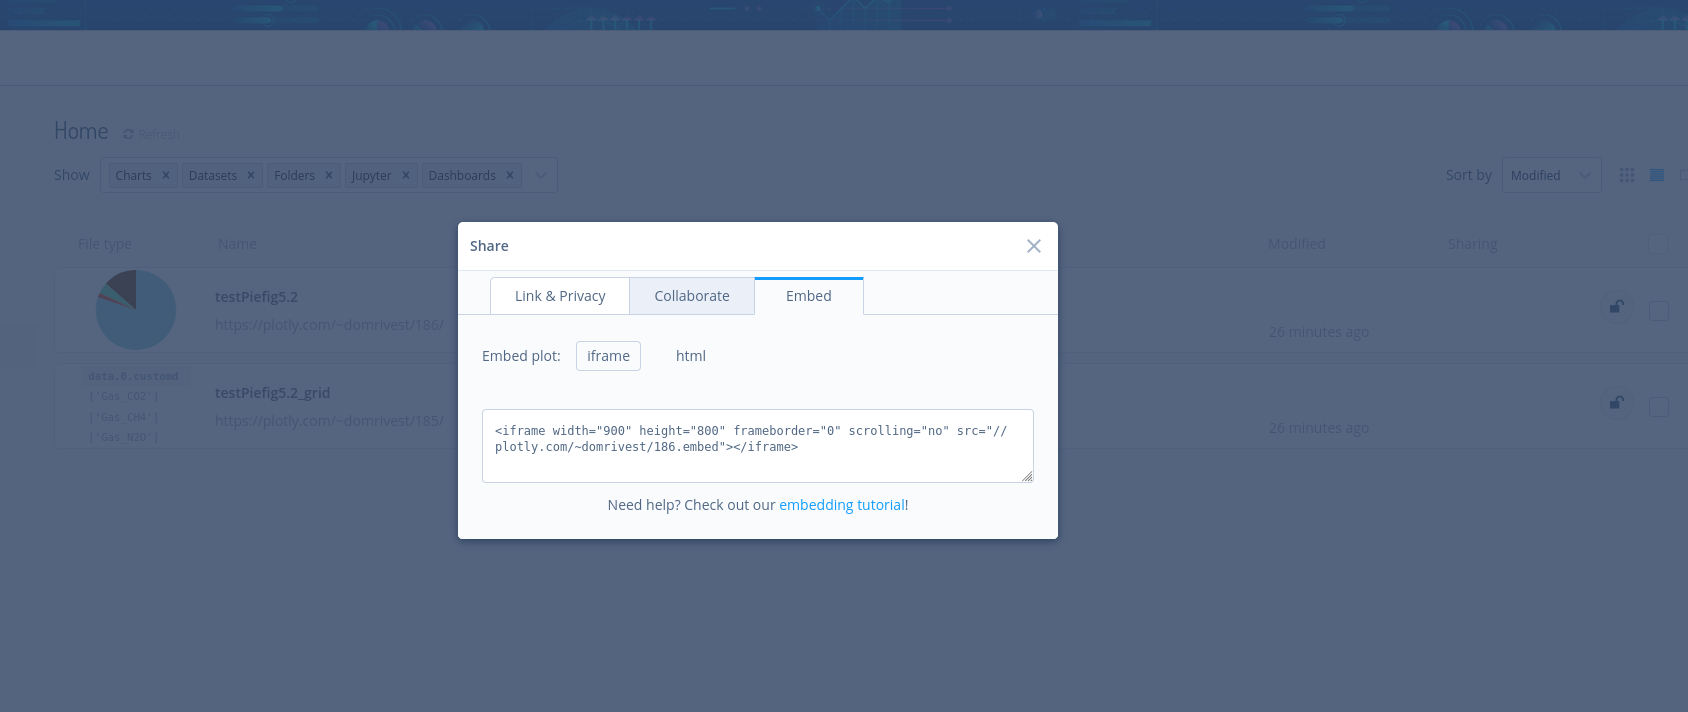
\includegraphics[width=\linewidth]{assets/chart-studio.png}
    \caption{Interface de chart-studio}
\end{figure}

\begin{figure}
    \includegraphics[width=\linewidth]{assets/intégrationWordpress.png}
    \caption{Intégration dans Wordpress}
\end{figure}

\end{document}